
%%% Local Variables: 
%%% mode: latex
%%% TeX-master: t
%%% End: 

\chapter{解码器并行优化}
\label{cha:parallelopt}

经过\refchapter{cha:singlecoreopt}的优化之后,我们的解码器性能仍然没有达到\refsec{sec:optaim}的要求。所以我们继续进行并行优化。本章主要从三个方面进行展开,首先\refsec{sec:parallelpossibility}分析解码器的并行性,然后\refsec{sec:parallelstructurebrief}介绍我们所实现的并行框架,最后\refsec{sec:parallelbuganddebug}说明并行中遇到的问题与解决方法。

\section{对解码器并行性的分析}
\label{sec:parallelpossibility}

在\refsec{sec:previouswork}中提到了H.264并行方向的一些研究\cite{li2005design,seitner2007macroblock,mesa2009scalability,yang2006parallel,ugur2007parallel}。虽然他们提出的具体方法我们没有采用,但是其思想与我们进行并行解码所做的思考是互通的。

解码过程中可能的并行性来自于两个方面:帧和宏块。

在解码帧的过程中,需要考虑参考结构。我们常常使用如\autoref{fig:mvcpredstructtyp}\footnote{图片选自\onlinecite{merkle2006efficient}中的Section 3}所示的参考结构。

\begin{figure}[htbp]
\begin{center}
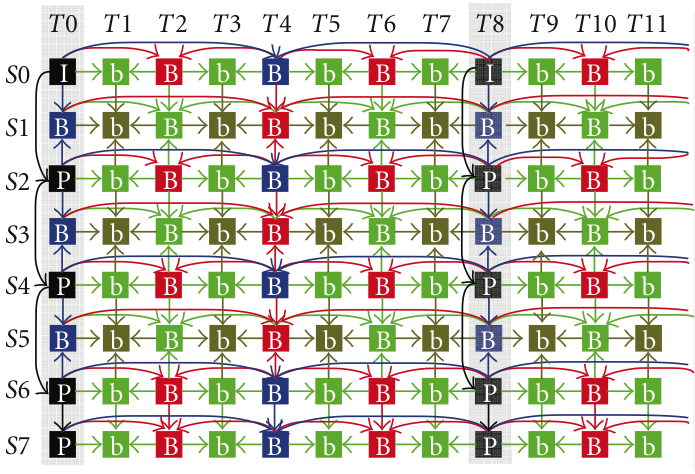
\includegraphics[width=0.7\textwidth]{mvcpredstructtyp.png}
\caption{典型的MVC参考结构}
\label{fig:mvcpredstructtyp}
\end{center}
\end{figure}

解码其中的I帧时,不需要参考任何帧,只要I帧的NAL Unit全部传入就可以开始对该帧解码。而对其中的P帧和B帧,都有箭头指向该帧,表示对这一帧的解码需要参考别的帧。我们用$(Sn,Tn)$表示在$Tn$时刻,$Sn$这一路码流对应的帧。$(S0,T1)$就需要参考$(S0,T0)$和$(S0,T2)$,而$(S0,T2)$又要参考$(S0,T0)$和$(S0,T4)$,$(S0,T4)$则要参考$(S0,T0)$和$(S0,T8)$,每一帧的解码都必须走过一条路径才能满足其参考帧都已经完成解码的条件。这样就形成了一个分层的图,从一个空的根节点向下,第i层的节点是第1到第i-1层解码完毕后立刻可以解码的帧。这样的图中,每一层的帧都可以并行地分别解码。如果将所有的视点$S0$到$S8$都考虑进来,情况就更加复杂。庞一等提出的多视点视频并行调度框架\cite{pang2009framework}就给出了这样的图的计算过程,对于\autoref{fig:goppredstructure}所示的预测结构,通过他们的算法能够得到如\autoref{fig:gopschedulinginmvc}所示的解码调度图\footnote{\autoref{fig:goppredstructure}和\autoref{fig:gopschedulinginmvc}分别选自\onlinecite{pang2009framework}的Section III与Section IV}。

\begin{figure}[htbp]
\begin{center}
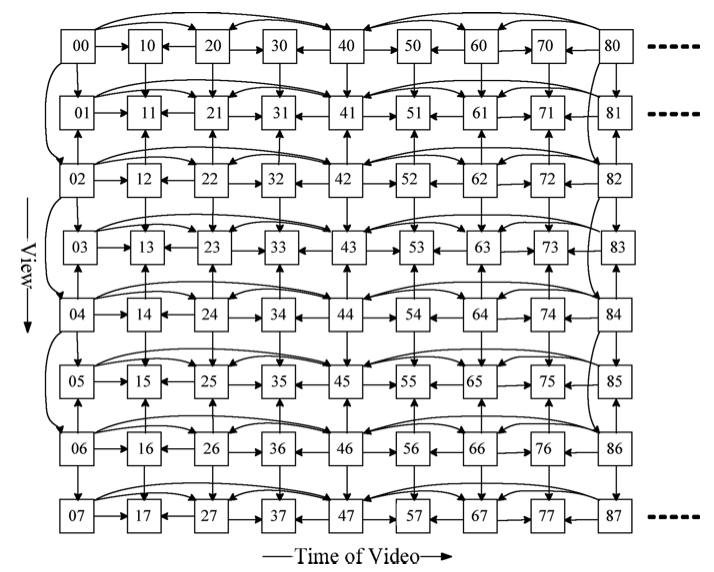
\includegraphics[width=0.7\textwidth]{goppredstructure.png}
\caption{GOP预测结构}
\label{fig:goppredstructure}
\end{center}
\end{figure}

\begin{figure}[htbp]
\begin{center}
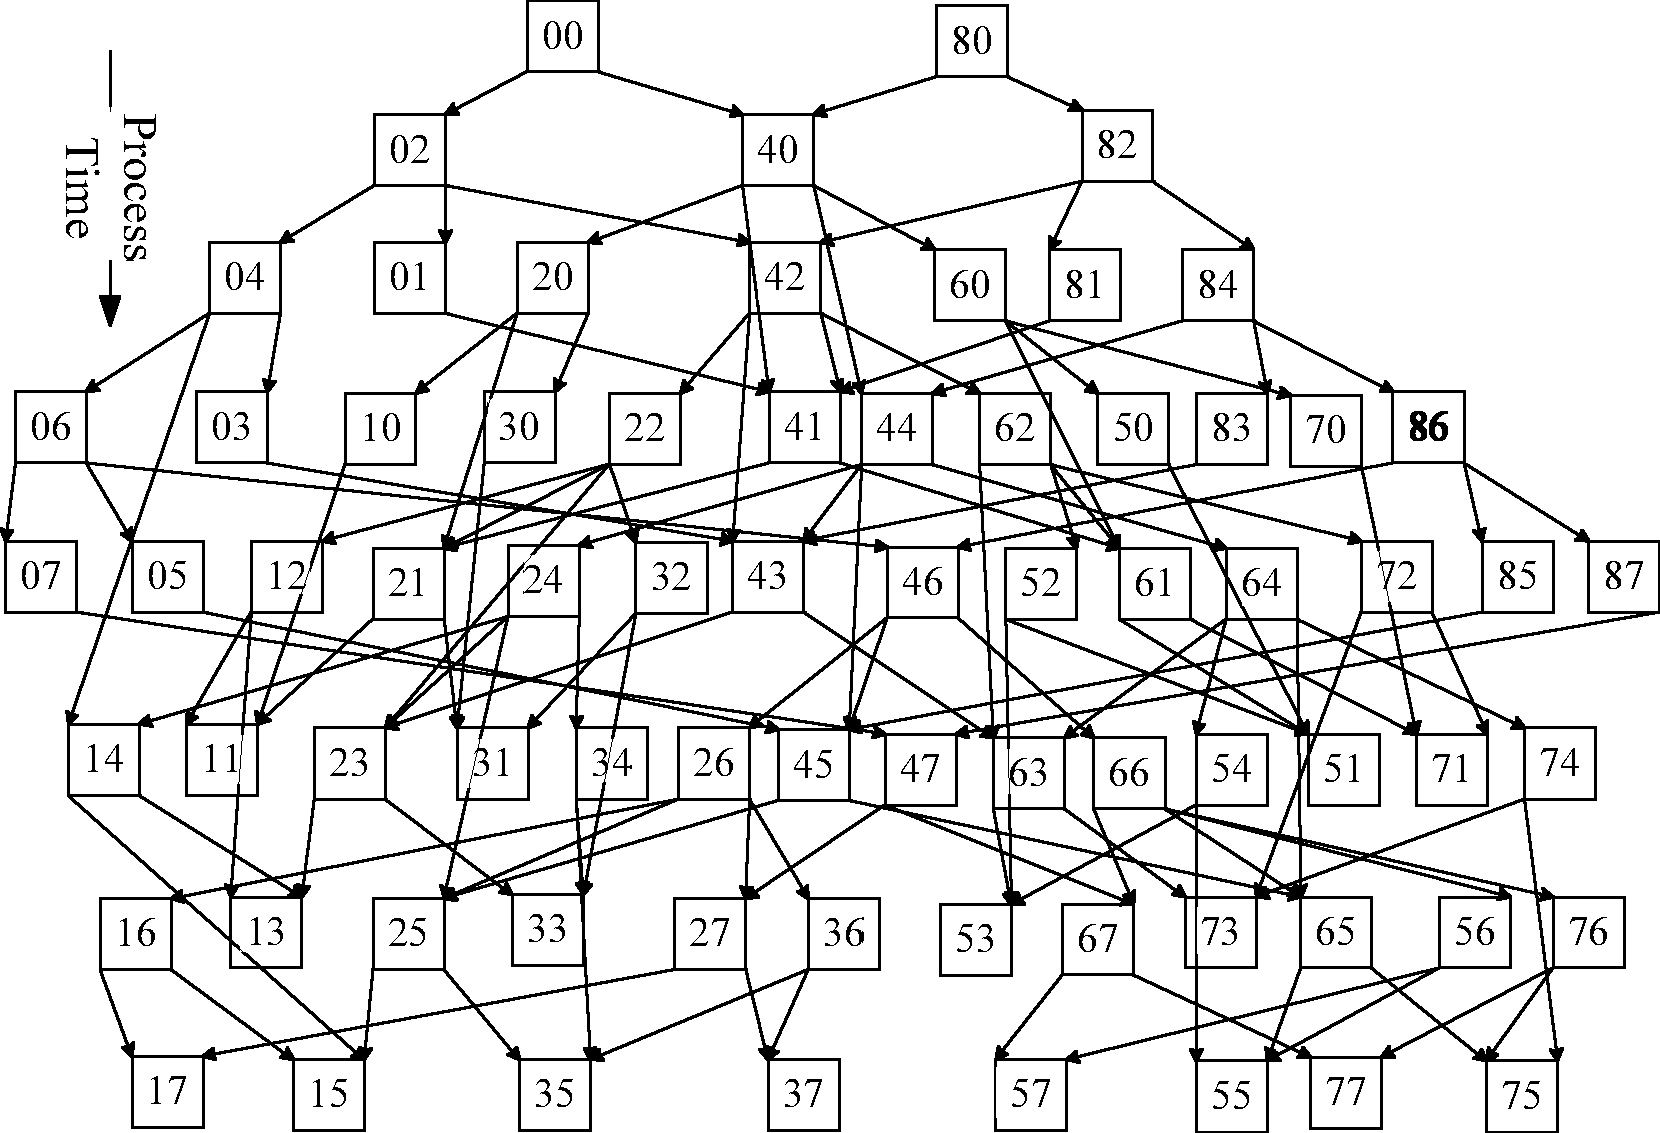
\includegraphics[width=0.8\textwidth]{gopschedulinginmvc.png}
\caption{多视点视频中的GOP调度}
\label{fig:gopschedulinginmvc}
\end{center}
\end{figure}

在解码宏块的过程中,也有相似参考结构,如\autoref{fig:mbparallelintra}\footnote{图片选自\onlinecite{meenderinck2009parallel}中的Section 4}所示。在解码$MB(4,1)$的时候,需要参考$MB(3,0)$、$MB(3,1)$、$MB(4,0)$的解码结果。从$T1$时刻解码左上角$MB(0,0)$起,$T2$时刻可以解码$MB(1,0)$,$T3$时刻可以同时解码$MB(2,0)$和$MB(0,1)$,$T4$可以同时解码$MB(3,0)$和$MB(1,1)$,以此类推。如果硬件资源足够同时解码3个宏块,那么全部16个宏块只要13个时间片就可以解码完成。

\begin{figure}[htbp]
\begin{center}
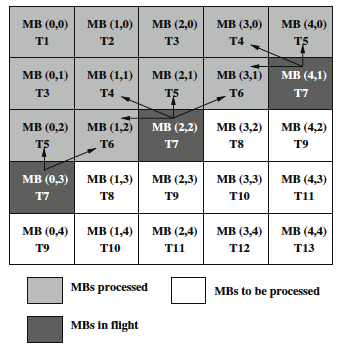
\includegraphics[width=0.6\textwidth]{mbparallelintra.png}
\caption{宏块参考结构}
\label{fig:mbparallelintra}
\end{center}
\end{figure}


\section{并行框架介绍}
\label{sec:parallelstructurebrief}

我们的解码器的框架如\autoref{fig:decoderModule}所示。有一个线程作为控制器控制整个解码器的工作,一个BitStreamReader线程负责读取源码流,一个RawDataWriter线程负责写解码后输出的码流。调度器就是\onlinecite{pang2009framework}中的算法实现,控制着1个到多个解码线程进行解码操作。可以看出,即使将解码线程的并行程度设为最多同时1个线程,整个解码器进程实际还是启用了多个线程的。

\begin{figure}[htbp]
\begin{center}
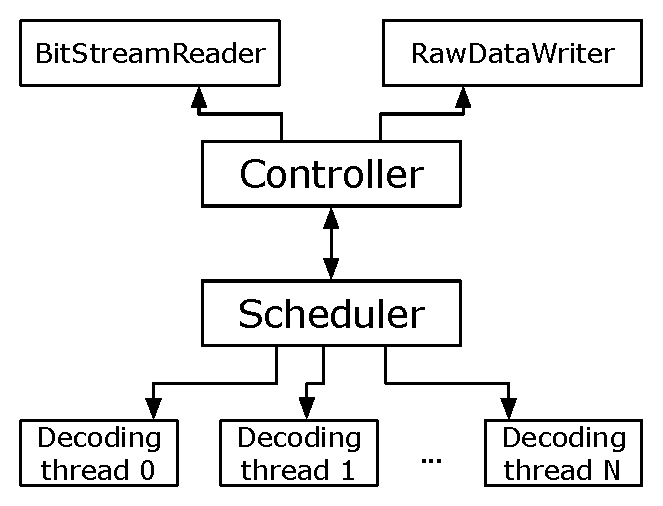
\includegraphics[width=0.5\textwidth]{decoderModule}
\caption{解码器模块关系}
\label{fig:decoderModule}
\end{center}
\end{figure}


\section{问题与解决}
\label{sec:parallelbuganddebug}

测试多线程解码的过程中,我们发现起初实现的版本在解码线程大于2的情况下,有不小的概率进入死锁状态,停滞在某一帧不前。这个概率随着解码线程数的增加而增大,在解码线程数为2的时候也有较小的概率进入这样的状态。这就令我们的并行解码实现失去了实用价值,我们不可能要求用户不断地尝试解码直到某次成功。

经过跟踪调试,我们找到了问题所在:在一些切换线程的位置上,我们使用了sleep(0)来暂停当前线程,希望回到控制线程。正是sleep(0)导致了程序停止后续任务的执行。过程如下
\begin{enumerate}
\item 读入一些NAL Unit,切换到解码线程
\item 解码线程发现数据不足以进行下一步解码,希望切回控制线程要求进一步数据
\item (这时应该置一个标志位通知控制线程做相应动作)
\item 但是此时没有同一优先级的线程希望获得资源,由于sleep(0)在其他线程不请求资源的情况下立即返回当前函数,而标志位尚未改变,于是就出现了死锁。
\end{enumerate}

将所有的sleep(0)改为 sleep(1)后,问题解决。经过查阅资料,我们发现,在Linux环境下,sleep(0)的确常被用于将cpu交给其他线程,但是在Windows下,经过测试发现sleep(0)会使cpu占用率接近100\%,所以实际上是一个死循环,没有其他任务的时候空消耗系统资源。

\section{小结}
\label{sec:sum5}

本章介绍了解码中存在的并行性,对帧并行和宏块并行都有所解释;之后说明了我们实现的解码器并行框架;最后提到了并行解码尝试中发现的一个问题和解决方法。